% !TEX root=../main.tex

\section{Top and TopHat}
\label{sec:tophat}

This section briefly introduces the task-oriented programming paradigm \TOP,
followed by a description of the task-oriented programming language \TOPHAT.



\subsection{TopHat}

TopHat (\TOPHAT) implements \TOP by embedding a task language in the simply typed lambda calculus with references, conditionals, primitive types and pairs.
Symbolic \TOPHAT extends this with \todo{Mention other features.}
References are used to model the shared data component of \TOP.
Below, the different components of \TOPHAT are explained in detail.
The complete syntax and semantics can be found in previous work~\cite{Steenvoorden2019}.


\subsubsection{Editors}

There are three different editors in \TOPHAT.
\begin{description}
  \item[$\Edit v$] Valued editor.\\
    This editor holds a value $v$ of a certain type.
    The user can replace the value by a new value of the same type.
  \item[$\Enter \tau$] Unvalued editor.\\
    This editor holds no value, and can receive a value of type $\tau$.
    When that happens, it turns into a valued editor.
  \item[$\Update l$] Shared editor.\\
    This editor refers to a store location $l$.
    Its observable value is the value stored at that location.
    When it receives a new value, this value will be stored at location $l$.
\end{description}


\subsubsection{Combinators}

The following combinators are available in \TOPHAT.
Here, $t$ stands for tasks and $e$ for arbitrary expressions.
\begin{description}
  \item[$t \Then e$] Step.\\
    Users can work on task $t$.
    As soon as $t$ has a value, that value is passed on to the right hand side $e$.
    The expression $e$ is a function, taking the value as an argument, resulting in a new task.
  \item[$t \Next e$] User Step.\\
    Users can work on task $t$.
    When $t$ has a value, the step becomes enabled.
    Users can then send a continue event to the combinator.
    When that happens, the value of $t$ is passed to the right hand side, with which it continues.
  \item[$t_1 \And t_2$] Composition.\\
    Users can work on tasks $t_1$ and $t_2$ in at the same time.
  \item[$t_1 \Or t_2$] Choice.\\
    The system chooses between $t_1$ or $t_2$,
    based on which task first has a value.
    If both tasks have a value, the system chooses the left one.
  \item[$e_1 \Xor e_2$] User choice.\\
    A user has to make a choice between either the left or the right hand side.
    The user continues to work on the chosen task.
\end{description}

In addition to editors and combinators, \TOPHAT also contains the fail task ($\Fail$).
Programmers can use this task to indicate that a task is not reachable or viable.
When the right hand side of a step combinator evaluates to $\Fail$, the step will not proceed to that task.

\todo{Say something about guarded tasks.}



\subsubsection{Observations}

Several observations can be made on tasks.
Using the value function $\Value$, the current value of a task can be determined.
The value function is a partial function, since not all tasks have a value.
For example empty editors and steps do not have a value.

One can also observe whether or not a task is failing, by means of the failing function $\Failing$.
The task $\Fail$ is failing, as is a parallel combination of failing tasks ($\Fail \And \Fail$).

The step combinator makes use of both functions in order to determine if it can step.
First, it uses $\Value$ to see if the left hand side produces a value.
If that is the case, it uses the $\Failing$ function to see if stepping to the right hand side is successful.

\begin{figure}[h]
  \centering \small
  \usemacro{O-Value}
  \caption{
    Value observation.
  } \label{}
\end{figure}

\subsubsection{Input}

Input events drive evaluation of tasks.
Because tasks are typed, input is typed as well.
Editors only accept input of the correct type.
Examples are replacing a value in an editor,
or sending a continue event to a user step.
When the system receives a valid event, it gives this event to the current task, which reduces to a new task.
Everything in between interaction steps is evaluated atomically with respect to inputs.
This means that tasks are normalised up to the point they await new user interactions.
% In this way the system communicates with the environment.

Input events are synchronous, which means the order of execution is completely determined by the order of the events.
In particular, the order of input events determine the progression of parallel branches.

\todo{Say something about the different semantics, since those will be used in a later section!}

\begin{figure}[h]
  \centering
  \includegraphics[width=0.8\columnwidth,page=5]{figures/drawings-crop.pdf}
  \caption{
    Semantic functions defined in this report and their relation.
  }
  \label{fig:semantic-functions}
\end{figure}

\boxed{\RelationE}
\boxed{\RelationS}
\boxed{\RelationN}
\boxed{\RelationH}
\boxed{\RelationI}

\begin{figure}[ht]
  \centering \small
  \usemacro{G-Values-Compact}
  \usemacro{G-Tasks-Compact}
  \caption{Syntax of values in \TOPHAT.}
  \label{fig:syntaxvalues}
\end{figure}
